% ==============================================================================
% TCC - Nome do Aluno
% Capítulo 2 - Referencial Teórico
% ==============================================================================
\chapter{Algoritmo de Dijkstra}
\label{sec-dijkstra}

\section{O Algoritmo}
\label{sec-dijkstra-algoritmo}
O algoritmo de Dijkstra tem por objetivo definir o menor caminho partindo do vértice origem $v_{s}$ e chegando a todos os demais vértices $v_{i}$ do grafo $G = (V,E)$. Para garantir a viabilidade do algoritmo, assume-se que todos os pesos $w( u, v )$ sejam maiores ou iguais a zero para toda aresta $E$ do grafo $G$ \cite{cormen2009introduction}.

A seguir é apresentado o pseudocódigo do algoritmo conforme descrito em \citeonline{drozdek2012data}.
%\begin{verbatim}
%CÓDIGO AQUI
%\end{verbatim}

\begin{lstlisting}[ mathescape, label=lst-dijkstra-codigo, caption=Algoritmo de Dijkstra., float=htpb]
DijkstraAlgorithm(weighted simple digraph, vertex first)
	for all vertices v
		currDist(v) = $\infty$;
	currDist(first) = 0;
	toBeChecked = all vertices;
	while toBeChecked is not empty
		v = a vertex in toBeChecked with minimal currDist(v);
		remove v from toBeChecked;
		for all vertices u adjacent to v and in toBeChecked
			if currDist( u ) > currDist( v ) + weight( edge(vu) )
				currDist( u ) = currDist( v ) + weight( edge(vu) );
				predecessor( u ) = v;
\end{lstlisting}

%\begin{verbatim}
%DijkstraAlgorithm(weighted simple digraph, vertex first)
%	for all vertices v
%	currDist(v) = infinite;
%	currDist(first) = 0;
%	toBeChecked = all vertices;
%	while toBeChecked is not empty
%		v = a vertex in toBeChecked with minimal currDist(v);
%		remove v from toBeChecked;
%		for all vertices u adjacent to v and in toBeChecked
%		if currDist( u ) > currDist( v ) + weight( edge(vu) )
%			currDist( u ) = currDist( v ) + weight( edge(vu) );
%			predecessor( u ) = v;
%\end{verbatim}

O algoritmo inicia atribuindo o valor inicial de cada distância de cada vértice do grafo igual a $\infty$ com exceção do vértice inicial $v_{s}$ que será iniciado por 0. Em seguida todos os vértices são adicionados ao conjunto dos "toBeChecked" ("aSeremChecados"). Feito isso, inicia-se o processo iterativo: seleciona-se o vértice $v$ de menor custo que esteja dentro do conjunto "toBeChecked", retira-se ele do conjunto e a partir dele, para cada vértice adjacente $u$ de $v$, verifica-se se a distância atual calculada de $u$ é maior do que a distância calculada de $v$ mais o valor referente ao peso da aresta de $v$ e $u$ (origem em $v$). Caso seja verdade, a distância atual de $u$ é substituída pela soma da distância atual de $v$ mais o peso da aresta de $v$ e $u$ (este valor corresponde a distância do vértice de origem $v_{s}$ até $u$), além de definir o antecessor $u$ como sendo $v$. Repete-se o passo iterativo até que o conjunto "toBeChecked" esteja vazio.

Ao final do algoritmo, teremos o conjunto de predecessores de cada vértice do grafo, e a partir deste, poderemos definir a rota para qualquer vértice do grafo partindo de $v_{s}$.\footnote{Em linguagens de programação, é costume substituir o valor $\infty$ pelo maior número representativo do tipo da variável selecionado para representar a distância. Por exemplo na linguagem C, caso se utilize o valor int (inteiro) para representar a distância, a atribuição inicial será dado pela constante INT\underline{\space}MAX  definida pela biblioteca "limits.h", que representa o maior valor numérico representado por esse tipo de variável.}

\begin{figure}[H]
\centering
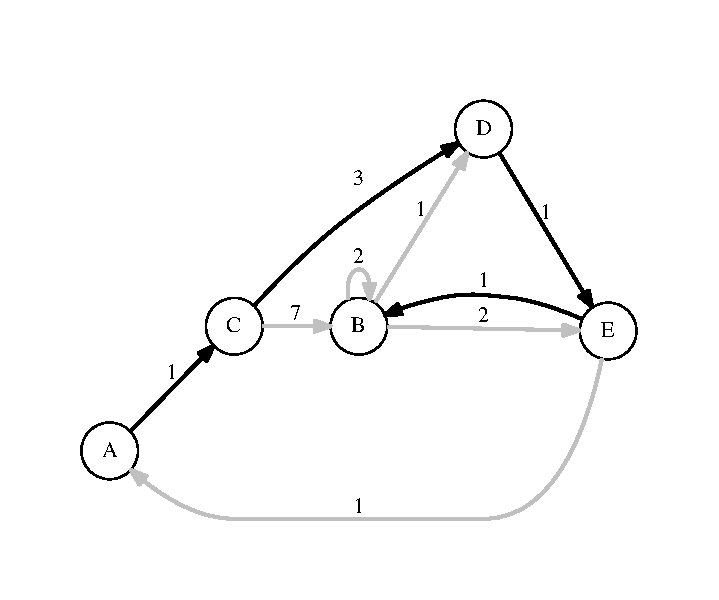
\includegraphics[width=1.\textwidth]{figuras/grafo-dijkstra} 
\caption{Aplicação do algoritmo de Dijkstra tendo o vértice "A" como origem. As arestas pintadas de preto correspondem a rota calculada a todos os demais vértices.}
\label{fig-dijkstra-algoritmo-grafo}
\end{figure}


\subsection{Garantia do algoritmo retorna o menor valor}
\label{sec-dijkstra-algoritmo-prova}
A prova será demonstrada em breve.

\section{Versões do Algoritmo implementadas e suas Estrutura de Dados}
\label{sec-dijkstra-versoes}
Para este projeto de graduação, será implementada três versões do algoritmo de Dijkstra baseados em estruturas de dados diversas que implicam em tempos computacionais diferentes \cite{cormen2009introduction}.

As versões implementadas são o Dijkstra Canônico, Dijkstra Heap Binário (seção \ref{sec-dijkstra-versoes-heap}) e Dijkstra Heap de Fibonacci (seção \ref{sec-dijkstra-versoes-fibonacci}), todas baseadas em \citeonline{cormen2009introduction, drozdek2012data}.

Para a versão Dijkstra Canônico, o algoritmo utiliza de um vetor para armazenar as distâncias calculadas pelo algoritmo (assim como os seus vértices correspondetes, que neste caso é utilizado o próprio indíce do vetor armazenado), e a cada passo iterativo (conforme demonstrado pelo algoritmo na seção \ref{sec-dijkstra-algoritmo}), uma busca linear é realizada para determinar o vértice (fora do conjunto "toBeChecked") cuja a distância é menor dentre todas as outras. O tempo computacional para esse caso é $O(|V^{2}|)$ \cite{drozdek2012data}.

\subsection{Dijkstra Heap Binário (A revisar)}
\label{sec-dijkstra-versoes-heap}
Para esta implementação, será utilizada a estrutura de dados heap binária mínima como fila de prioridade. Heaps binária podem ser descritas como árvores binárias que possuem as seguintes propriedades \cite{drozdek2012data}:
\begin{enumerate}
 \item O valor de cada nodo não é maior do que os valores guardados em cada um de seus filhos.
 \item A árvore é perfeitamente balanceada, e as folhas no último nível estão todas mais a esquerda.
\end{enumerate}

Um exemplo de estrutura Heap Binário representada tanto como árvore como vetor pode ser visualizado nas figuras \ref{fig-dijkstra-heapbinario} e \ref{fig-dijkstra-heapvetor} respectivamente.

\begin{figure}[H]
\centering
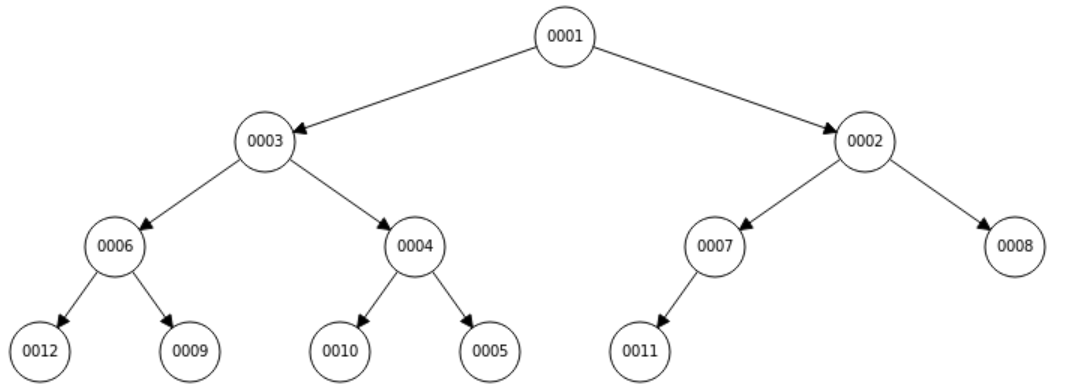
\includegraphics[width=.95\textwidth]{figuras/Heap} 
\caption{Exemplo de Heap Binário representado como árvore.}
\label{fig-dijkstra-heapbinario}
\end{figure}

\begin{figure}[H]
\centering
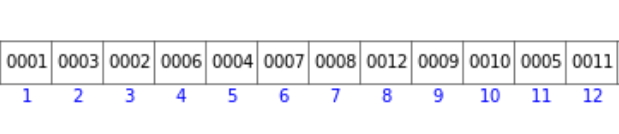
\includegraphics[width=.60\textwidth]{figuras/Heap-vetor}
\caption{Representação do Heap Binário da figura \ref{fig-dijkstra-heapbinario} como vetor.}
\label{fig-dijkstra-heapvetor}
\end{figure}

A disposição dos elementos da árvore no vetor segue as seguintes relações entre nós pai, filho-direita e filho-esquerda:
%\begin{equation}
%Pai(i): \lfloor i/2 \rfloor
%\end{equation}
%\begin{equation}
%Filho-esquerda(i): 2*i
%\end{equation}
%\begin{equation}
%Filho-direita(i): 2*i+1
%\end{equation}
\begin{description}
\item[Pai($i$):] $\lfloor i/2 \rfloor$
\item[Filho-esquerda($i$):] $2*i$
\item[Filho-direita($i$):] $2*i+1$
\end{description}
Onde $i \in \mathbb{N}$ e $i \subset [1, n]$, sendo que $i$ representa o índice do elemento no vetor e $n$ o número de elementos da árvore.

 Para efeitos de exemplo (observe as figuras \ref{fig-dijkstra-heapbinario} e \ref{fig-dijkstra-heapvetor} para constatação), o nó que está contido na posição 4 do vetor, possuí como pai o nó de posição 2 ($\lfloor 4 / 2 \rfloor = 2$) e tem como filho da esquerda o nó de posição 8 ($2*4 = 8$) e filho da direita o nó de posição 9 ($2*4+1 = 9$).

%\begin{equation}
%\forall i, i \in \mathbb{N} [1,n]
%\end{equation}

A vantagem de se usar essa estrutura de dados reside no fato de suas operações de inserção, extração de mínimo e reconstrução da heap possuirem tempo computacional de $O(\log n)$. Por consequência, o tempo computacional para este caso é de $O(|E| \log |V|)$ \cite{cormen2009introduction}.

\subsection{Dijkstra Heap de Fibonacci}
\label{sec-dijkstra-versoes-fibonacci}


\section{Experimentos Computacionais}
\label{sec-dijkstra-experimentos}
Para a realização dos experimentos computacionais será rodado instâncias de grafos que representam malhas rodoviárias reais. Todas elas descritas nas tabelas \ref{tbl-dijkstra-instancias} e \ref{tbl-dijkstra-configuracao}, e disponíveis no sítio eletrônico \url{http://www.dis.uniroma1.it/challenge9/download.shtml} (acesso em 28 de janeiro de 2017).
\begin{table}[H]
\caption{Instâncias a serem rodadas pelo algoritmo de Dijkstra em suas três versões.}
\label{tbl-dijkstra-instancias}
\centering
\begin{adjustbox}{max width=\textwidth}
\begin{tabular}{|c|c|}
\hline 
\textbf{Nome Instância} & \textbf{Descrição} \\ 
\hline 
USA-road-d.NY.gr & Representa a malha viária do estado de Nova Iorque, Estados Unidos \\ 
\hline 
USA-road-d.BAY.gr & Representa a malha viária da bahia de São Francisco, Califórnia, Estados Unidos \\ 
\hline 
USA-road-d.COL.gr & Representa a malha viária do estado do Colorado, Estados Unidos \\ 
\hline 
USA-road-d.FLA.gr & Representa a malha viária do estado da Flórida, Estados Unidos \\ 
\hline 
\end{tabular}
\end{adjustbox}
\end{table}

\begin{table}[H]
\caption{Configuração dos grafos correspondestes as malhas viárias descritas na tabela \ref{tbl-dijkstra-instancias}.}
\label{tbl-dijkstra-configuracao}
\centering
\begin{adjustbox}{max width=\textwidth}
\begin{tabular}{|c|c|c|}
\hline 
\textbf{Nome Instância} & \textbf{Número de Vértices |V|} & \textbf{Número de Arestas |E|} \\ 
\hline 
USA-road-d.NY.gr
 & 264.346
 & 733.846
 \\ 
\hline 
USA-road-d.BAY.gr
 & 321.270
 & 800.172
 \\ 
\hline 
USA-road-d.COL.gr
 & 435.666
 & 1.057.066
 \\ 
\hline 
USA-road-d.FLA.gr
 & 1.070.376
 & 2.712.798
 \\ 
\hline 
\end{tabular}
\end{adjustbox} 
\end{table}

\subsection{Resultados obtidos}
\label{sec-dijkstra-experimentos-resultados}
Os resultados dos testes podem ser descritos a seguir.

\begin{figure}[H]
\centering
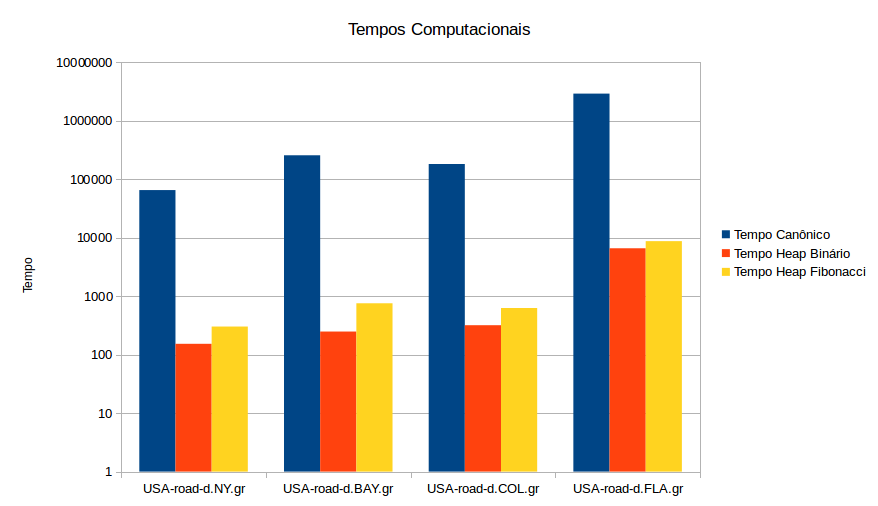
\includegraphics[width=.90\textwidth]{figuras/dijkstra-tempos} 
\caption{Tempos computacionais obtidos pelos Métodos de Dijkstra empregados (tempo em escala logarítmica).}
\label{fig-dijkstra-resultados-tempos}
\end{figure}

\begin{figure}[H]
\centering
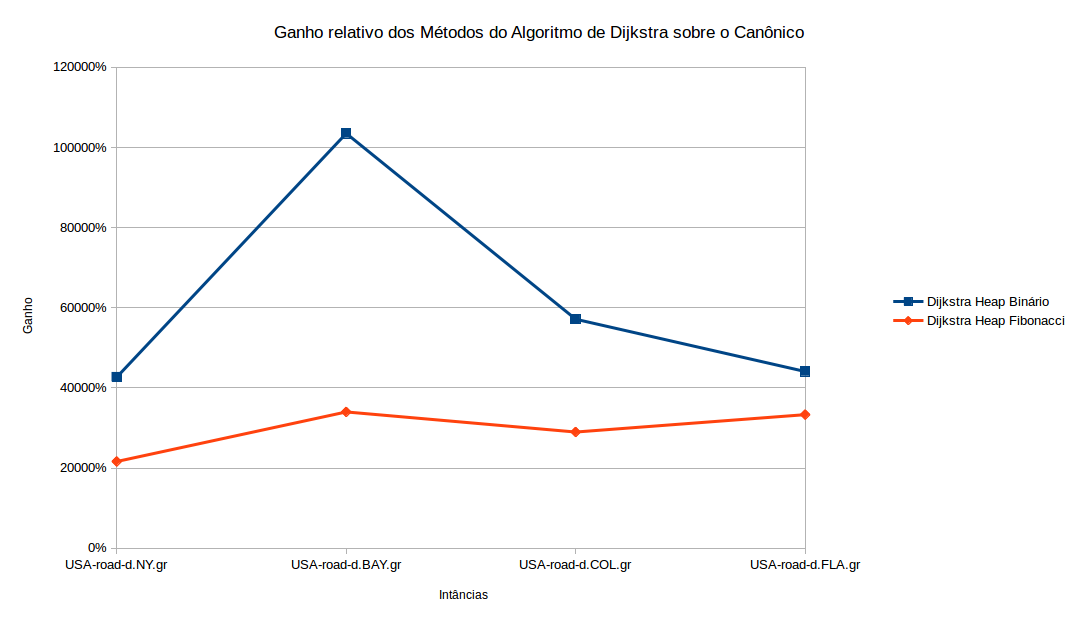
\includegraphics[width=.90\textwidth]{figuras/speed-up-dijkstra} 
\caption{Ganho relativo dos Métodos do Algoritmo de Dijkstra sobre o Canônico.}
\label{fig-dijkstra-resultados-speedup}
\end{figure}


\begin{table}[H]
\caption{Tempos Computacionais obtidos pelo algoritmo de Dijkstra em suas diferentes versões (tempo em milissegundos).}
\label{tbl-dijkstra-resultados-tempos}
\centering
\begin{adjustbox}{max width=\textwidth}
\begin{tabular}{|c|c|c|c|}
\hline
\textbf{Nome Instância} & \textbf{Tempo Canônico} & \textbf{Tempo Heap Binário} & \textbf{Tempo Heap Fibonacci} \\ \hline
USA-road-d.NY.gr        & 65287                   & 153                         & 302                           \\ \hline
USA-road-d.BAY.gr       & 256690                  & 248                         & 755                           \\ \hline
USA-road-d.COL.gr       & 181687                  & 318                         & 627                           \\ \hline
USA-road-d.FLA.gr       & 2909655                 & 6601                        & 8732                          \\ \hline
\end{tabular}
\end{adjustbox}
\end{table}


\begin{table}[H]
\caption{Ganho relativo sobre o Dijkstra Canônico.}
\label{tbl-dijkstra-resultados-speedup}
\centering
\begin{adjustbox}{max width=\textwidth}
\begin{tabular}{|c|c|c|}
\hline
\textbf{Nome Instância} & \textbf{Ganho Heap Binário} & \textbf{Ganho Heap Fibonacci} \\ \hline
USA-road-d.NY.gr        & 42.671\%                       & 21.618\%                         \\ \hline
USA-road-d.BAY.gr       & 103.504\%                      & 33.999\%                         \\ \hline
USA-road-d.COL.gr       & 57.134\%                       & 28.977\%                         \\ \hline
USA-road-d.FLA.gr       & 44.079\%                       & 33.322\%                         \\ \hline
\end{tabular}
\end{adjustbox}
\end{table}

\subsection{Análise dos resultados}
\label{sec-dijkstra-experimentos-analise}


\section{Conclusões}
\label{sec-dijkstra-conclusoes}
Conforme apresentado por \citeonline{larkin2014back}.